%% using aastex version 6.3
\documentclass[preprint2]{aastex63}

%% The default is a single spaced, 10 point font, single spaced article.
%% There are 5 other style options available via an optional argument. They
%% can be invoked like this:
%%
%% \documentclass[arguments]{aastex63}
%% 
%% where the layout options are:
%%
%%  twocolumn   : two text columns, 10 point font, single spaced article.
%%                This is the most compact and represent the final published
%%                derived PDF copy of the accepted manuscript from the publisher
%%  manuscript  : one text column, 12 point font, double spaced article.
%%  preprint    : one text column, 12 point font, single spaced article.  
%%  preprint2   : two text columns, 12 point font, single spaced article.
%%  modern      : a stylish, single text column, 12 point font, article with
%% 		  wider left and right margins. This uses the Daniel
%% 		  Foreman-Mackey and David Hogg design.
%%  RNAAS       : Preferred style for Research Notes which are by design 
%%                lacking an abstract and brief. DO NOT use \begin{abstract}
%%                and \end{abstract} with this style.
%%
%% Note that you can submit to the AAS Journals in any of these 6 styles.
%%
%% There are other optional arguments one can invoke to allow other stylistic
%% actions. The available options are:
%%
%%   astrosymb    : Loads Astrosymb font and define \astrocommands. 
%%   tighten      : Makes baselineskip slightly smaller, only works with 
%%                  the twocolumn substyle.
%%   times        : uses times font instead of the default
%%   linenumbers  : turn on lineno package.
%%   trackchanges : required to see the revision mark up and print its output
%%   longauthor   : Do not use the more compressed footnote style (default) for 
%%                  the author/collaboration/affiliations. Instead print all
%%                  affiliation information after each name. Creates a much 
%%                  longer author list but may be desirable for short 
%%                  author papers.
%% twocolappendix : make 2 column appendix.
%%   anonymous    : Do not show the authors, affiliations and acknowledgments 
%%                  for dual anonymous review.
%%
%% these can be used in any combination, e.g.
%%
%% \documentclass[twocolumn,linenumbers,trackchanges]{aastex63}
%%
%% AASTeX v6.* now includes \hyperref support. While we have built in specific
%% defaults into the classfile you can manually override them with the
%% \hypersetup command. For example,
%%
%% \hypersetup{linkcolor=red,citecolor=green,filecolor=cyan,urlcolor=magenta}
%%
%% will change the color of the internal links to red, the links to the
%% bibliography to green, the file links to cyan, and the external links to
%% magenta. Additional information on \hyperref options can be found here:
%% https://www.tug.org/applications/hyperref/manual.html#x1-40003
%%
%% Note that in v6.3 "bookmarks" has been changed to "true" in hyperref
%% to improve the accessibility of the compiled pdf file.
%%
%% If you want to create your own macros, you can do so
%% using \newcommand. Your macros should appear before
%% the \begin{document} command.
%%
\usepackage{xfrac}
\usepackage{amsmath}
\usepackage{upgreek}

\newcommand{\vdag}{(v)^\dagger}
\newcommand\aastex{AAS\TeX}
\newcommand\latex{La\TeX}
\newcommand\Rm{{\rm Rm} }
\newcommand\Rey{{\rm Re} }
\newcommand\Pm{{\rm Pm} }
\newcommand\kf{k_{\rm f} }
\newcommand\SNr{\dot\sigma_{\rm sn}}
\newcommand\OSN{\Omega_{\rm sn}}
\newcommand\ESK{E_{\rm kin}}
\newcommand\EST{E_{\rm th}}
\newcommand\ESN{E_{\sigma}}
\newcommand\Ms{M_{\rm s}}
\newcommand{\vect}[1]{{{\mbox{\boldmath $#1$}}}}%also makes bold Greek letters
\newcommand{\mathbfss}[1]{\textbf{\textsf{#1}}}
\newcommand\kpc{~ {\rm kpc}}
\newcommand\pc{~ {\rm pc}}
\newcommand\dx{ {\delta x}}
\newcommand\Myr{~ {\rm Myr}}
\newcommand\erg{~ {\rm erg}}
\newcommand\kms{~ {\rm km~ s}^{-1}}
\newcommand\BKM{{\color{blue}{BKMM4}}}

\definecolor{midblue}{rgb}{0.0,0.4,0.7}
\definecolor{midgreen}{rgb}{0.1,0.6,0.3}
\definecolor{mypurple}{rgb}{0.7,0.3,0.8}
\newcommand{\fg}[1]{\textcolor{mypurple}{#1}}
\newcommand{\mm}[1]{\textcolor{mypurple}{#1}}
\newcommand{\fag}[1]{\textcolor{midblue}{FAG: #1}}
\newcommand{\ns}[1]{\textcolor{orange}{#1}}
\newcommand{\mjk}[1]{\textcolor{red}{#1}}

%% Reintroduced the \received and \accepted commands from AASTeX v5.2
\received{October 4, 2020}
\revised{\today}
\accepted{}
%% Command to document which AAS Journal the manuscript was submitted to.
%% Adds "Submitted to " the argument.
\submitjournal{ApJL}

%% For manuscript that include authors in collaborations, AASTeX v6.3
%% builds on the \collaboration command to allow greater freedom to 
%% keep the traditional author+affiliation information but only show
%% subsets. The \collaboration command now must appear AFTER the group
%% of authors in the collaboration and it takes TWO arguments. The last
%% is still the collaboration identifier. The text given in this
%% argument is what will be shown in the manuscript. The first argument
%% is the number of author above the \collaboration command to show with
%% the collaboration text. If there are authors that are not part of any
%% collaboration the \nocollaboration command is used. This command takes
%% one argument which is also the number of authors above to show. A
%% dashed line is shown to indicate no collaboration. This example manuscript
%% shows how these commands work to display specific set of authors 
%% on the front page.
%%
%% For manuscript without any need to use \collaboration the 
%% \AuthorCollaborationLimit command from v6.2 can still be used to 
%% show a subset of authors.
%
%\AuthorCollaborationLimit=2
%
%% will only show Schwarz & Muench on the front page of the manuscript
%% (assuming the \collaboration and \nocollaboration commands are
%% commented out).
%%
%% Note that all of the author will be shown in the published article.
%% This feature is meant to be used prior to acceptance to make the
%% front end of a long author article more manageable. Please do not use
%% this functionality for manuscripts with less than 20 authors. Conversely,
%% please do use this when the number of authors exceeds 40.
%%
%% Use \allauthors at the manuscript end to show the full author list.
%% This command should only be used with \AuthorCollaborationLimit is used.

%% The following command can be used to set the latex table counters.  It
%% is needed in this document because it uses a mix of latex tabular and
%% AASTeX deluxetables.  In general it should not be needed.
%\setcounter{table}{1}

%%%%%%%%%%%%%%%%%%%%%%%%%%%%%%%%%%%%%%%%%%%%%%%%%%%%%%%%%%%%%%%%%%%%%%%%%%%%%%%%
%%
%% The following section outlines numerous optional output that
%% can be displayed in the front matter or as running meta-data.
%%
%% If you wish, you may supply running head information, although
%% this information may be modified by the editorial offices.
\shorttitle{Fluctuating small-scale dynamo modes}
\shortauthors{Gent et al.}
%%
%% You can add a light gray and diagonal water-mark to the first page 
%% with this command:
%% \watermark{text}
%% where "text", e.g. DRAFT, is the text to appear.  If the text is 
%% long you can control the water-mark size with:
%% \setwatermarkfontsize{dimension}
%% where dimension is any recognized LaTeX dimension, e.g. pt, in, etc.
%%
%%%%%%%%%%%%%%%%%%%%%%%%%%%%%%%%%%%%%%%%%%%%%%%%%%%%%%%%%%%%%%%%%%%%%%%%%%%%%%%%

%% This is the end of the preamble.  Indicate the beginning of the
%% manuscript itself with \begin{document}.

\begin{document}

\title{Fluctuating small-scale dynamo modes in supernova driven multi-phase turbulence}

%%
%% The \author command is the same as before except it now takes an optional
%% argument which is the 16 digit ORCID. The syntax is:
%% \author[xxxx-xxxx-xxxx-xxxx]{Author Name}
%%
%%
%% Use \affiliation for affiliation information. The old \affil is now aliased
%% to \affiliation. AASTeX v6.3 will automatically index these in the header.
%% When a duplicate is found its index will be the same as its previous entry.
%%
%% Note that \altaffilmark and \altaffiltext have been removed and thus 
%% can not be used to document secondary affiliations. If they are used latex
%% will issue a specific error message and quit. Please use multiple 
%% \affiliation calls for to document more than one affiliation.
%%
%% The new \altaffiliation can be used to indicate some secondary information
%% such as fellowships. This command produces a non-numeric footnote that is
%% set away from the numeric \affiliation footnotes.  NOTE that if an
%% \altaffiliation command is used it must come BEFORE the \affiliation call,
%% right after the \author command, in order to place the footnotes in
%% the proper location.
%%
%% Use \email to set provide email addresses. Each \email will appear on its
%% own line so you can put multiple email address in one \email call. A new
%% \correspondingauthor command is available in V6.3 to identify the
%% corresponding author of the manuscript. It is the author's responsibility
%% to make sure this name is also in the author list.
%%
%% While authors can be grouped inside the same \author and \affiliation
%% commands it is better to have a single author for each. This allows for
%% one to exploit all the new benefits and should make book-keeping easier.
%%
%% If done correctly the peer review system will be able to
%% automatically put the author and affiliation information from the manuscript
%% and save the corresponding author the trouble of entering it by hand.

\correspondingauthor{Maarit K\"apyl\"a}
\email{Email: frederick.gent@aalto.fi, mordecai@amnh.org,\\ maarit.kapyla@aalto.fi, nishant@iucaa.in}

\author[0000-0002-1331-2260]{Frederick A. Gent}
\affiliation{
Astroinformatics, Department of Computer Science, Aalto University, P.O. Box 15400, FI-00076 Espoo, Finland
 }
\affiliation{
    School of Mathematics, Statistics and Physics,
      Newcastle University, NE1 7RU, UK 
 }

\author[0000-0003-0064-4060]{Mordecai-Mark {Mac Low}}
\affiliation{
  Department of Astrophysics, {79th Street at Central Park West, }American Museum of Natural History,
  New York, NY 10024, USA
}
\affiliation{
{Center for Computational Astrophysics, {162 Fifth Avenue, }Flatiron Institute, New York,
NY 10010, USA} 
}

\author[0000-0002-9614-2200]{Maarit J. K\"apyl\"a}
\affiliation{
Astroinformatics, Department of Computer Science, Aalto University, P.O. Box 15400, FI-00076 Espoo, Finland
}
\affiliation{
Max Planck Institute for Solar System Research, Justus-von-Liebig-Weg 3, D-37707 G\"ottingen, Germany
}
\affiliation{
    Nordic Institute for Theoretical Physics,
      Roslagstullsbacken 23, SE-106 91 Stockholm, Sweden 
}

\author[0000-0001-6097-688X]{Nishant K. Singh}
\affiliation{
Inter-University Centre for Astronomy \& Astrophysics, Post Bag 4, Ganeshkhind, Pune 411 007, India
}
\affiliation{
Max Planck Institute for Solar System Research, Justus-von-Liebig-Weg 3, 37707 G\"ottingen, Germany
}

%% AASTeX 6.3 has the new \collaboration and \nocollaboration commands to
%% provide the collaboration status of a group of authors. These commands 
%% can be used either before or after the list of corresponding authors. The
%% argument for \collaboration is the collaboration identifier. Authors are
%% encouraged to surround collaboration identifiers with ()s. The 
%% \nocollaboration command takes no argument and exists to indicate that
%% the nearby authors are not part of surrounding collaborations.

%% Mark off the abstract in the ``abstract'' environment. 
\begin{abstract}
Magnetic fields grow quickly even at early cosmological times, suggesting the
action of a small-scale dynamo (SSD) in the interstellar medium of galaxies.
Many studies have focused on idealized turbulent driving of the SSD. 
Here we simulate more realistic supernova-driven turbulence to determine
whether it can drive an SSD.
Magnetic field growth occurring in our models appears inconsistent with simple
tangling of magnetic fields, but consistent with SSD action, reproducing and
confirming models by \citet{BKMM04} that did not include physical resistivity
$\eta$.
We vary $\eta$, as well as the numerical resolution and supernova rate,
$\dot\sigma$, to delineate the regime in which an SSD occurs.
For a given $\dot\sigma$ we find convergence for SSD growth rate with
resolution of a parsec.
For $\dot\sigma\simeq\dot\sigma_{\rm sn}$, with $\dot\sigma_{\rm sn}$ the solar
neighborhood rate, the critical resistivity below which an SSD occurs is
$0.005>\eta_{\rm crit}>0.001\,\rm kpc\,\rm km~ s^{-1}$, and this
increases with the supernova rate.
Across the modeled range of 0.5--4 pc resolution we find that for
$\eta<\eta_{\rm crit}$, the SSD saturates at about 5\% of kinetic energy
equipartition, independent of growth rate.
In the range $0.2\,\dot\sigma_{\rm sn}\leq\dot\sigma\leq8\,\dot\sigma_{\rm sn}$
growth rate increases with $\dot\sigma$.
SSDs in the supernova-driven interstellar medium commonly exhibit erratic
growth.
\end{abstract}
\keywords{dynamo --- magnetohydrodynamics (MHD) --- ISM: supernova remnants --- ISM: magnetic fields --- turbulence}


\section{Introduction}\label{sec:intro}
%==============================================================================

%---------------------------------------------------------------------------
\section[]{Shock tests}
\label{sect:shocks}

%---------------------------------------------------------------------------

%-------------------------------------------------------------------------
\begin{figure*}
\centering
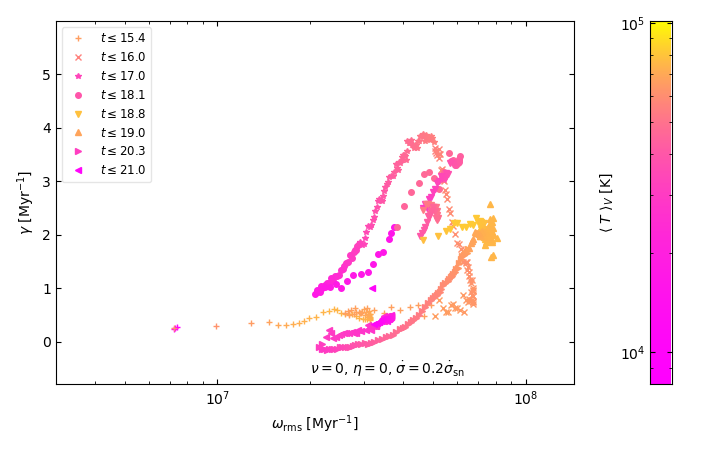
\includegraphics[trim=0.2cm 1.4cm 0.5cm 0.2cm,clip=true,width=0.49\textwidth]{csc_figs/gvw-0.5pcPm0e-0.0.png}
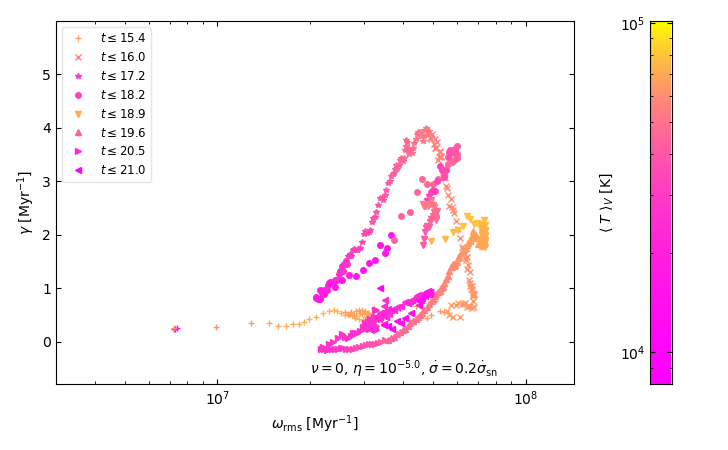
\includegraphics[trim=0.2cm 1.4cm 0.5cm 0.2cm,clip=true,width=0.49\textwidth]{csc_figs/gvw-0.5pcPm0e-5.0.png}
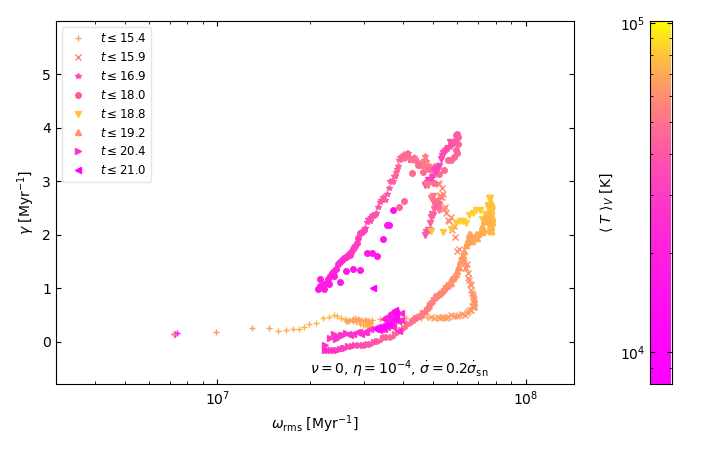
\includegraphics[trim=0.2cm 0.2cm 0.5cm 0.2cm,clip=true,width=0.49\textwidth]{csc_figs/gvw-0.5pcPm0e-4.0.png}
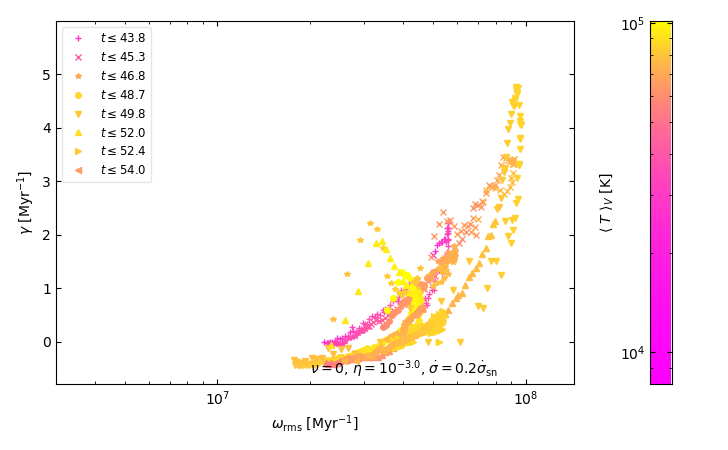
\includegraphics[trim=0.2cm 0.2cm 0.5cm 0.2cm,clip=true,width=0.49\textwidth]{csc_figs/gvw-0.5pcPm0e-3.0.png}
  \begin{picture}(0,0)(0,0)
  %  \put(-452,544){{\sf{$\delta x=0.5$}}}
  %  \put(-452,531){{\sf{$\dot\sigma=\frac{1}{5}\SNr$}}}
  %  \put(-205,544){{\sf{$\delta x=1$}}}
  %  \put(-205,531){{\sf{$\nu=10^{-3}$}}}
  %  \put(-205,518){{\sf{$\dot\sigma=\frac{1}{5}\SNr$}}}
  %  \put(-452,415){{\sf{$\delta x=1$}}}
  %  \put(-452,402){{\sf{$\dot\sigma=\frac{1}{5}\SNr$}}}
  %  \put(-205,415){{\sf{$\delta x=1$}}}
  %  \put(-205,402){{\sf{$\eta=10^{-4}$}}}
  %  \put(-205,389){{\sf{$\dot\sigma=\frac{1}{5}\SNr$}}}
  %  \put(-452,260){{\sf{$\delta x=2$}}}
  %  \put(-452,247){{\sf{$\dot\sigma=\frac{1}{5}\SNr$}}}
  %  \put(-205,260){{\sf{$\delta x=4$}}}
  %  \put(-205,247){{\sf{$\dot\sigma=\frac{1}{5}\SNr$}}}
  %  \put(-452,133){{\sf{$\delta x=2$}}}
  %  \put(-452,120){{\sf{$\dot\sigma=\SNr$}}}
  %  \put(-205,133){{\sf{$\delta x=4$}}}
  %  \put(-205,120){{\sf{$\dot\sigma=\SNr$}}}
    \put(-395,205){{\sf\bf{(a)}}}
    \put(-225,205){{\sf\bf{(b)}}}
    \put(-395, 35){{\sf\bf{(c)}}}
    \put(-225, 35){{\sf\bf{(d)}}}
  \end{picture}
\caption{
Growth rate vs rms vorticity with volumetric mean temperature indicated by 
color for $\dx=0.5$.
Symbols indicated in the legend apply during the time intervals listed.
\label{fig:lsd-power}
}
\end{figure*}
%--------------------------------------------------------------------------

%-------------------------------------------------------------------------
\begin{figure*}
\centering
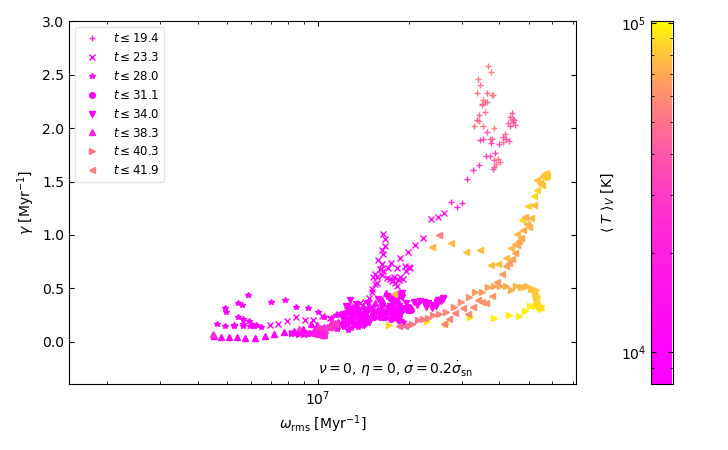
\includegraphics[trim=0.2cm 1.4cm 0.5cm 0.2cm,clip=true,width=0.49\textwidth]{csc_figs/gvw-1pcPm0e-0.0.png}
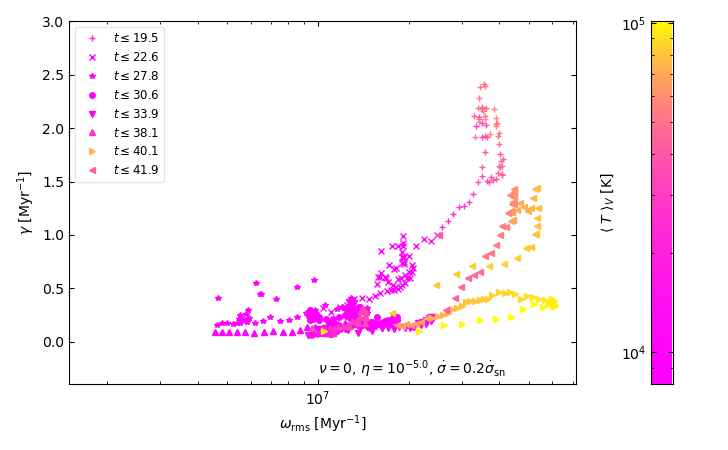
\includegraphics[trim=0.2cm 1.4cm 0.5cm 0.2cm,clip=true,width=0.49\textwidth]{csc_figs/gvw-1pcPm0e-5.0.png}
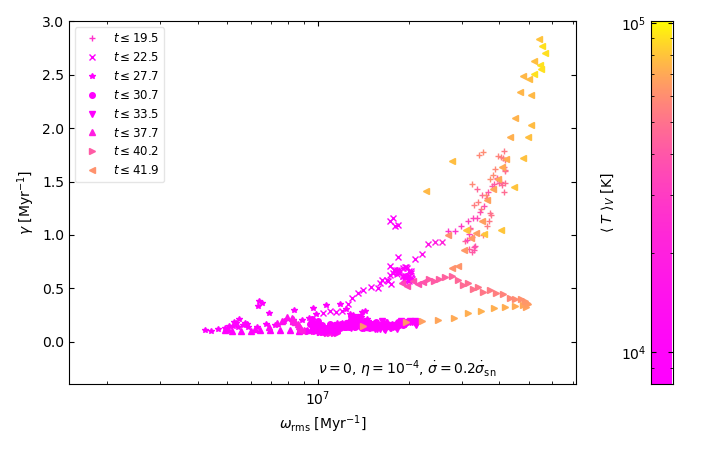
\includegraphics[trim=0.2cm 0.2cm 0.5cm 0.2cm,clip=true,width=0.49\textwidth]{csc_figs/gvw-1pcPm0e-4.0.png}
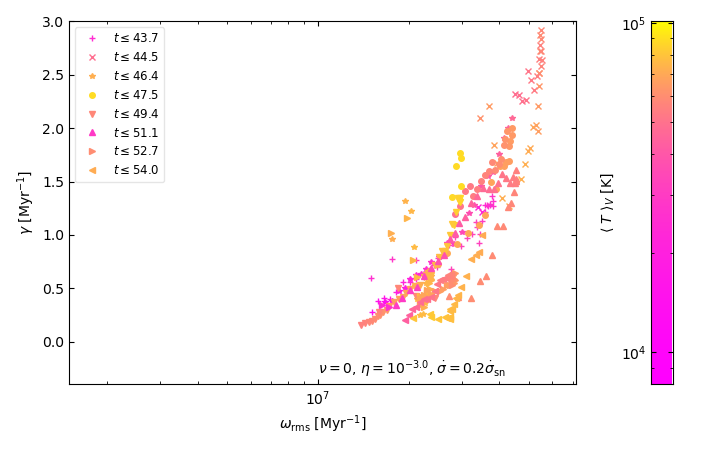
\includegraphics[trim=0.2cm 0.2cm 0.5cm 0.2cm,clip=true,width=0.49\textwidth]{csc_figs/gvw-1pcPm0e-3.0.png}
\caption{
Growth rate vs rms vorticity with volumetric mean temperature indicated by 
color for $\dx=1$.
Symbols indicated in the legend apply during the time intervals listed.
\label{fig:lsd-power}
}
\end{figure*}
%--------------------------------------------------------------------------


%-------------------------------------------------------------------------
\begin{figure*}
\centering
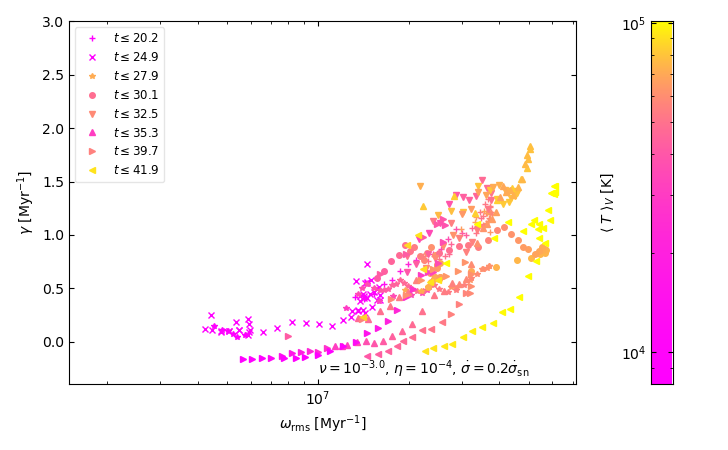
\includegraphics[trim=0.2cm 1.4cm 0.5cm 0.2cm,clip=true,width=0.49\textwidth]{csc_figs/gvw-1pcPm10e-4.0.png}
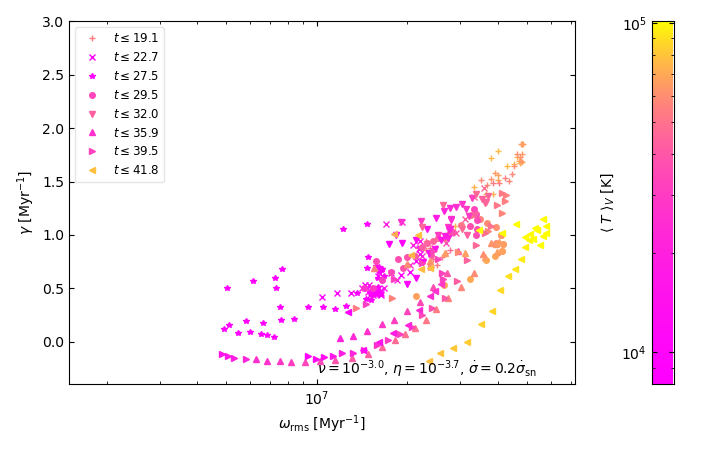
\includegraphics[trim=0.2cm 1.4cm 0.5cm 0.2cm,clip=true,width=0.49\textwidth]{csc_figs/gvw-1pcPm5e-3.7.png}
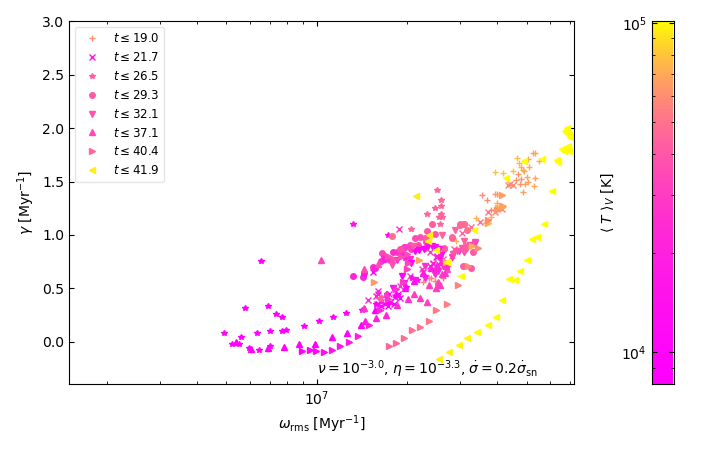
\includegraphics[trim=0.2cm 0.2cm 0.5cm 0.2cm,clip=true,width=0.49\textwidth]{csc_figs/gvw-1pcPm2e-3.3.png}
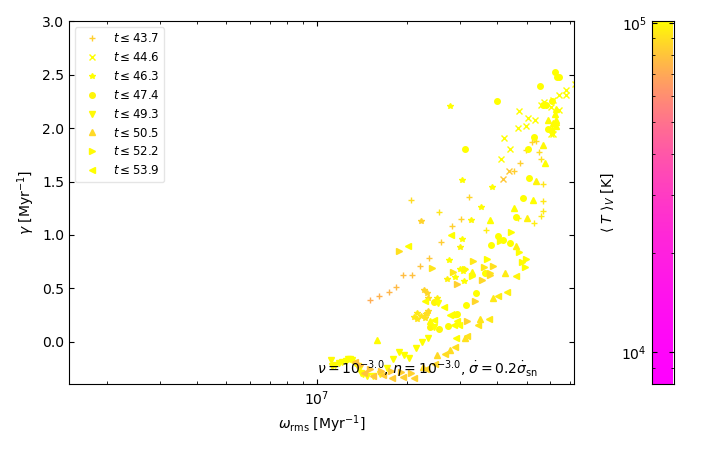
\includegraphics[trim=0.2cm 0.2cm 0.5cm 0.2cm,clip=true,width=0.49\textwidth]{csc_figs/gvw-1pcPm1e-3.0.png}
\caption{
Growth rate vs rms vorticity with volumetric mean temperature indicated by 
color for $\dx=1$.
Symbols indicated in the legend apply during the time intervals listed.
\label{fig:lsd-power}
}
\end{figure*}
%--------------------------------------------------------------------------

%-------------------------------------------------------------------------------

 We solve the system of nonideal, compressible, nonisothermal MHD equations
%-------------------------------------------------------------------------------
  \begin{eqnarray}
  \label{eq:mass}
    \frac{D\rho}{Dt} &=& 
    -\rho \vect\nabla \cdot \vect{u}
    +\vect\nabla \cdot\zeta_D\vect\nabla\rho,
  \end{eqnarray}
%-------------------------------------------------------------------------------
  \begin{eqnarray}
  \label{eq:mom}
    \rho\frac{D\vect{u}}{Dt} &=& 
    \vect\nabla{\ESK\sigma}
    -\rho c_{\rm s}^2\vect\nabla\left({s}/{c_{\rm p}}+\ln\rho\right)
    +\vect{j}\times\vect{B}
    \nonumber\\
    &+&\vect\nabla\cdot \left(2\rho\nu{\mathbfss W}\right)
    +\rho\,\vect\nabla\left(\zeta_{\nu}\vect\nabla \cdot \vect{u} \right)
    \nonumber\\
    &+&\vect\nabla\cdot \left(2\rho\nu_3{\mathbfss W}^{(3)}\right)
  {-\vect u\vect{\nabla}\cdot\left(\zeta_D\vect{\nabla}\rho\right)},
  \end{eqnarray}
%-------------------------------------------------------------------------------
  \begin{eqnarray}
  \label{eq:ent}
    \rho T\frac{D s}{Dt} &=&
     \EST\dot\sigma +\rho\Gamma
    -\rho^2\Lambda +\eta\mu_0\vect{j}^2 
    \nonumber\\
    &+&2 \rho \nu\left|{\mathbfss W}\right|^{2}
    +\rho\,\zeta_{\nu}\left(\vect\nabla \cdot \vect{u} \right)^2
    \nonumber\\
    &+&\vect\nabla\cdot\left(\zeta_\chi\rho T\vect\nabla s\right)
    +\rho T\chi_3\vect\nabla^6 s
    \nonumber\\
    &-& {c_{\rm{v}}\,T \left(
    \zeta_D\nabla^2\rho + \vect\nabla\zeta_D\cdot\vect\nabla\rho\right)},
  \end{eqnarray}
%-------------------------------------------------------------------------------
  \begin{eqnarray}
  \label{eq:ind}
    \frac{\partial \vect{A}}{\partial t} &=&
    \vect{u}\times\vect{B}
    +\eta\vect\nabla^2\vect{A}
    +\eta_3\vect\nabla^6\vect{A},
  \end{eqnarray}
%-------------------------------------------------------------------------------
 with the ideal gas equation of state closing the system.
 Most variables take their usual meanings.
 Terms containing $\zeta_D{=2},\,\zeta_\nu=5$ and $\zeta{_\chi=2}$
 {are applied to all ISM models and} resolve shock discontinuities with
 artificial diffusion of mass, momentum, and energy proportional to shock
 strength \citep[see][for details]{GMKSH20}.
 {Equations~\eqref{eq:mom} and \eqref{eq:ent} include terms with $\zeta_D$}
 {to} {provide momentum and energy conserving corrections for} {the}
 {artificial mass diffusion applying in Equation~\eqref{eq:mass}.}
 {In previous work \citet{Gent:2013b} we have used a formalism that
 included artificial diffusion in vector potential at shocks.
 %Shock diffusion is not applied to Equation~\eqref{eq:ind}{, unlike} {in}
 %{\citet{Gent:2013b}.}
 %This avoids {excessive magnetic dissipation in
 %  shocks, where compression actually enhances it.}
 In Figure~\ref{fig:eb-slice} we show comparative slices of the magnetic
 energy and gas density with and without resistive shock diffusion
 $\zeta_\eta$.
 With $\zeta_\eta>0$ (Fig.~\ref{fig:eb-slice} b) magnetic energy is reduced in the remnant shell relative to Figure~\ref{fig:eb-slice} a, where compression actually enhances it.}
 Since the magnetic field is well resolved in either case, as also
 shown by the magnetic energy spectra below, and the simulation is
 numerically stable without it, this extra artificial
 diffusion is unnecessary.

 In both models a concentration of magnetic energy, marked with $+$ in
 Figure\,\ref{fig:eb-slice}, has below average gas density.
 {This snapshot reflects the overall behavior of the system, in which
 magnetic field amplification also occurs independently of shock compression.
 As Figure\,\ref{fig:eb-slice} shows, SN shock fronts do compress and amplify
 the magnetic field, resulting in strong local and instantaneous correlation
 of the field and density.
 However, on global and long-term scales, this is not the dominant mechanism
 for the dynamo, which operates just as effectively in the nonshocked, more
 diffuse regions, as is also indicated by this figure.
 This is based on the amplification factor due to compression being estimated
 $\lesssim2$, taken as density fluctuations to power $4/3$, while the magnetic
 energy is amplified by 4--6 orders of magnitude.}

  {Unlike past} experiments \citep{Gent:2013b,Gent:2013a,GMKSH20},
 thermal diffusivity $\chi$ is {also} omitted, as the artificial diffusivities
 {chosen} are adequate to ensure numerical stability.
 {The} physical effects of thermal conductivity can be expected to be
 relevant only at the unresolved or marginally resolved Field length defined
 by \citet[][named after George Field, not the magnetic field]{BM90}.
 Terms containing $\nu_3,\,\chi_3$ and $\eta_3$ apply sixth-order hyperdiffusion
 to resolve grid-scale instabilities \citep[see, e.g.,][]{ABGS02,HB04}, {
 with mesh Reynolds number set to be $\simeq1$ for each $\dx$}.

 The simplified isothermal model considered in
Sect.\,\ref{sec:ssd-tang} solves only Equations~\eqref{eq:mass},
 \eqref{eq:mom}, and~\eqref{eq:ind}, without the shock-dependent diffusion or
 hyperdiffusion terms, and while setting
 $\vect{B}=\vect\nabla\times\vect{A}+\vect{B}_{\rm imposed}$.

 {In the ISM simulations} SNe are exploded at {uniform} random positions
 at a Poisson rate $\dot\sigma$ {scaled by} the solar neighborhood
 value $\SNr\simeq 50\kpc^{-3}\Myr^{-1}$.
 Explosions inject $\EST = 10^{51}\erg$ thermal energy, except in
 dense regions, where a proportion ($<5\%$) may be kinetic $\ESK$ 
 \citep[see][]{GMKSH20}.
 {Models with common $\dot\sigma$ have the same timing and location of
 explosions.}
 Nonadiabatic heating $\Gamma$ and cooling $\Lambda (T)$ are included
 \citep{Gent:2013b} following \citet{Wolfire:1995} and \citet{Sarazin:1987}.

%-------------------------------------------------------------------------
\begin{figure*}
\centering
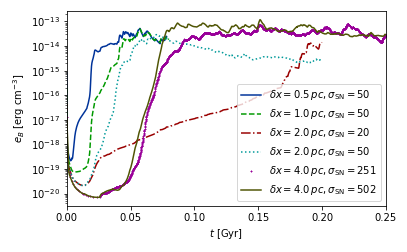
\includegraphics[trim=0.0cm 0.0cm 0.0cm 0.0cm,clip=true,width=0.47\textwidth]{csc_figs/sn_dx.png}
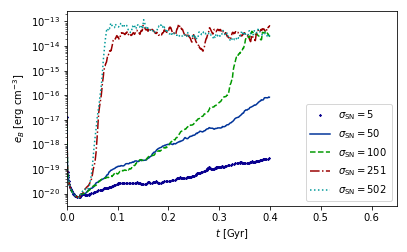
\includegraphics[trim=0.0cm 0.0cm 0.0cm 0.0cm,clip=true,width=0.47\textwidth]{csc_figs/sn4pc.png}
\caption{
Effect of supernova rate, $\sigma_{\rm SN}$ [kpc$^{-3}$Myr$^{-1}$], at various
spatial resolution. Panel (b) 4\,pc with $\sigma_{\rm SN} \in[5,502]$.
{Remember to comment that we compared constant heating vs \citet{Wolfire:1995} et al and this was not significant.}
\label{fig:brms_SNrate}
}
\end{figure*}
%-------------------------------------------------------------------------

%-------------------------------------------------------------------------
\begin{figure}
\centering
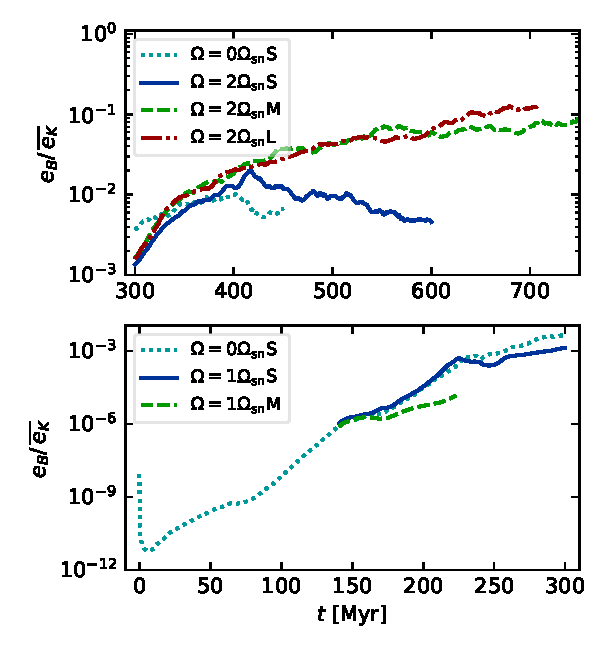
\includegraphics[trim=0.0cm 0.0cm 0.0cm 0.0cm,clip=true,width=0.45\textwidth]{csc_figs/eB-res-4eta.pdf}
\caption{
Magnetic energy density, $e_B$, normalised by time averaged kinetic energy 
density, $\overline{e_K}$, at $\dx=4$\,pc with rotation rate $\Omega$ as
indicated in the legends, and shear ratio $q=1.5$ (upper) and 1 (lower). 
Legend labels S, M and L indicate azimuthal length $Ly=0.512,\,1.024$ and 
1.536\,kpc, respectively. 
\label{fig:lsd-eB}
}
\end{figure}
%--------------------------------------------------------------------------

%------------------------------------------------------------------------- 
\begin{table*}
\caption{\texttt{*} indicates simulation data lost}
\begin{tabular}{lccccccc}
Model             & resolution & $\eta_3,\nu_3$      & $\nu$            & $\eta$          & $\dot\sigma$ & \\
                  & [pc]       &                     & [kpc km s$^{-1}$]&[kpc km s$^{-1}$]&[$\dot\sigma_{\rm SN}$]& \\
\texttt{uPm0e-0.0sn02}  & 0.5 & 3.25$\cdot10^{-16}$ &                  &                 &  0.2  \\
\texttt{uPm0e-5.0sn02}  & 0.5 & 3.25$\cdot10^{-16}$ &                  & $     10^{-5}$  &  0.2  \\
\texttt{uPm0e-4.0sn02}  & 0.5 & 3.25$\cdot10^{-16}$ &                  & $     10^{-4}$  &  0.2  \\
\texttt{uPm0e-3.0sn02}  & 0.5 & 3.25$\cdot10^{-16}$ &                  & $     10^{-3}$  &  0.2  \\
\texttt{hPm0e-0.0sn02}   & 1.0 & 3.5$\cdot10^{-15}$  &                  &                 &  0.2  \\
\texttt{hPm0e-5.0sn02}   & 1.0 & 3.5$\cdot10^{-15}$  &                  &                 &  0.2  \\
\texttt{hPm0e-4.0sn02}   & 1.0 & 3.5$\cdot10^{-15}$  &                  & $      10^{-3}$ &  0.2  \\
\texttt{hPm0e-3.0sn02}   & 1.0 & 3.5$\cdot10^{-15}$  &                  & $      10^{-4}$ &  0.2  \\
\texttt{hPm001e-4.0sn02} & 1.0 & 3.5$\cdot10^{-15}$  & $      10^{-6}$  & $      10^{-4}$ &  0.2  \\
\texttt{hPm01e-4.0sn02  }& 1.0 & 3.5$\cdot10^{-15}$  & $      10^{-5}$  & $      10^{-4}$ &  0.2  \\
\texttt{hPm02e-4.0sn02  }& 1.0 & 3.5$\cdot10^{-15}$  & $2\cdot10^{-5}$  & $      10^{-4}$ &  0.2  \\
\texttt{hPm05e-4.0sn02  }& 1.0 & 3.5$\cdot10^{-15}$  & $5\cdot10^{-5}$  & $      10^{-4}$ &  0.2  \\
\texttt{hPm02e-2.3sn02  }& 1.0 & 3.5$\cdot10^{-15}$  & $      10^{-3}$  & $5\cdot10^{-3}$ &  0.2  \\
\texttt{hPm1e-4.0sn02  } & 1.0 & 3.5$\cdot10^{-15}$  & $      10^{-4}$  & $      10^{-4}$ &  0.2  \\
\texttt{hPm1e-3.0sn02  } & 1.0 & 2.5$\cdot10^{-15}$  & $      10^{-3}$  & $      10^{-3}$ &  0.2  \\
\texttt{hPm2e-3.3sn02  } & 1.0 & 2.5$\cdot10^{-15}$  & $      10^{-3}$  & $      10^{-3}$ &  0.2  \\
\texttt{hPm5e-3.7sn02  } & 1.0 & 2.5$\cdot10^{-15}$  & $      10^{-3}$  & $5\cdot10^{-4}$ &  0.2  \\
\texttt{hPm5e-4.0sn02  } & 1.0 & 3.5$\cdot10^{-15}$  & $5\cdot10^{-4}$  & $2\cdot10^{-4}$ &  0.2  \\
\texttt{hPm10e-4.0sn02  }& 1.0 & 3.5$\cdot10^{-15}$  & $      10^{-3}$  & $      10^{-4}$ &  0.2  \\
\texttt{hPm10e-4.0sn02-Z}& 1.0 & 3.5$\cdot10^{-15}$  & $      10^{-3}$  & $      10^{-4}$ &  0.2  \\
\texttt{hPm5e-3.1sn05}   & 1.0 & 3.5$\cdot10^{-15}$  & $4\cdot10^{-3}$  & $8\cdot10^{-4}$ &  0.5  \\
\texttt{hPm5e-3.1sn05-L} & 1.0 & 3.5$\cdot10^{-15}$  & $4\cdot10^{-3}$  & $8\cdot10^{-4}$ &  0.5  \\
\texttt{cPm2.5e4.0sn8-B} &0.78 & 3.5$\cdot10^{-15}$  &$2.5\cdot10^{-4}$ & $      10^{-4}$ &  8.0  \\
\texttt{cPm2.5e4.0sn8-B} &1.56 & 3.5$\cdot10^{-15}$  &$2.5\cdot10^{-4}$ & $      10^{-4}$ &  8.0  \\
\texttt{cPm0e4.0sn8-B}   &1.56 & 3.5$\cdot10^{-15}$  &                  & $      10^{-4}$ &  8.0  
\end{tabular}
\end{table*}
\begin{table*}
\caption{\texttt{*} indicates simulation data lost}
\begin{tabular}{lccccccc}
Model             & resolution & $\eta_3,\nu_3$      & $\nu$            & $\eta$          & $\dot\sigma$ & \\
                  & [pc]       &                     & [kpc km s$^{-1}$]&[kpc km s$^{-1}$]&[$\dot\sigma_{\rm SN}$]& \\
\texttt{mPm0e-0.0sn1}    & 2.0 & 8.25$\cdot10^{-14}$ &                  &                 &  0.4 \\
\texttt{mPm0e-0.0sn1}    & 2.0 & 8.25$\cdot10^{-14}$ &                  &                 &  1.0 \\
\texttt{mPm0e-6.0sn1}    & 2.0 & 8.25$\cdot10^{-14}$ &                  & $     10^{-6}$  &  1.0 \\
\texttt{mPm0e-5.0sn1}    & 2.0 & 8.25$\cdot10^{-14}$ &                  & $     10^{-5}$  &  1.0 \\
\texttt{mPm0e-4.0sn1}    & 2.0 & 8.25$\cdot10^{-14}$ &                  & $     10^{-4}$  &  1.0 \\
\texttt{mPm0e-3.3sn1}    & 2.0 & 8.25$\cdot10^{-14}$ &                  & 5$\cdot10^{-4}$ &  1.0 \\
\texttt{mPm0e-3.0sn1}    & 2.0 & 8.25$\cdot10^{-14}$ &                  & $     10^{-3}$  &  1.0 \\
\texttt{mPm0e-0.0sn02}   & 2.0 & 8.25$\cdot10^{-14}$ &                  &                 &  0.2 \\
\texttt{mPm0e-4.0sn02}   & 2.0 & 8.25$\cdot10^{-14}$ &                  & $     10^{-4}$  &  0.2 \\
\texttt{mPm0e-3.0sn02}   & 2.0 & 8.25$\cdot10^{-14}$ &                  & $     10^{-3}$  &  0.2 \\
\texttt{mPm1e-4.0sn1}    & 2.0 & 8.25$\cdot10^{-14}$ & $     10^{-4}$   & $     10^{-4}$  &  1.0 \\
\texttt{mPm1e-4.0sn02}   & 2.0 & 8.25$\cdot10^{-14}$ & $     10^{-4}$   & $     10^{-4}$  &  0.2 \\
\texttt{mPm1e-4.0sn02-B} & 2.0 & 8.25$\cdot10^{-14}$ & $     10^{-4}$   & $     10^{-4}$  &  0.2 \\
\texttt{mPm05e-4.0sn1}   & 2.0 & 8.25$\cdot10^{-14}$ & 5$\cdot10^{-5}$  & $     10^{-4}$  &  1.0 \\
\texttt{mPm05e-4.0sn02}  & 2.0 & 8.25$\cdot10^{-14}$ & 5$\cdot10^{-5}$  & $     10^{-4}$  &  0.2 \\
\texttt{mPm02e-4.0sn1}   & 2.0 & 8.25$\cdot10^{-14}$ & 2$\cdot10^{-5}$  & $     10^{-4}$  &  1.0 \\
\texttt{mPm02e-4.0sn02}  & 2.0 & 8.25$\cdot10^{-14}$ & 2$\cdot10^{-5}$  & $     10^{-4}$  &  0.2 \\
\texttt{mPm01e-4.0sn1}   & 2.0 & 8.25$\cdot10^{-14}$ & $     10^{-5}$   & $     10^{-4}$  &  1.0 \\
\texttt{mPm01e-4.0sn02}  & 2.0 & 8.25$\cdot10^{-14}$ &       $10^{-5}$  & $     10^{-4}$  &  0.2 
\end{tabular}
\end{table*}
\begin{table*}
\caption{\texttt{*} indicates simulation data lost}
\begin{tabular}{lccccccc}
Model            & resolution & $\eta_3,\nu_3$      & $\nu$            & $\eta$          & $\dot\sigma$  \\
                 & [pc]       &                     & [kpc km s$^{-1}$]&[kpc km s$^{-1}$]&[$\dot\sigma_{\rm SN}$] \\
\texttt{lPm0e-0.0sn01}  & 4.0 & 2$\cdot10^{-12}$    &                  &                 & 0.1  \\
\texttt{lPm0e-0.0sn2}   & 4.0 & 2$\cdot10^{-12}$    &                  &                 & 2.0  \\
\texttt{lPm0e-0.0sn5}   & 4.0 & 2$\cdot10^{-12}$    &                  &                 & 5.0  \\
\texttt{lPm0e-0.0sn10}  & 4.0 & 2$\cdot10^{-12}$    &                  &                 & 10.0 \\
\texttt{lPm0e-0.0sn1}   & 4.0 & 2$\cdot10^{-12}$    &                  &                 &  1.0 \\
\texttt{lPm0e-6.0sn1}   & 4.0 & 2$\cdot10^{-12}$    &                  & $     10^{-6}$  &  1.0 \\
\texttt{lPm0e-5.0sn1}   & 4.0 & 2$\cdot10^{-12}$    &                  & $     10^{-5}$  &  1.0 \\
\texttt{lPm0e-4.0sn1}   & 4.0 & 2$\cdot10^{-12}$    &                  & $     10^{-4}$  &  1.0 \\
\texttt{lPm0e-3.7sn1}   & 4.0 & 2$\cdot10^{-12}$    &                  & 2$\cdot10^{-4}$ &  1.0 \\
\texttt{lPm0e-3.3sn1}   & 4.0 & 2$\cdot10^{-12}$    &                  & 5$\cdot10^{-3}$ &  1.0 \\
\texttt{lPm0e-3.0sn1}   & 4.0 & 2$\cdot10^{-12}$    &                  & $     10^{-3}$  &  1.0 \\
\texttt{lPm0e-3.3sn1}   & 4.0 & 2$\cdot10^{-12}$    &                  & 5$\cdot10^{-4}$ &  1.0 \\
\texttt{lPm0e-2.3sn1}   & 4.0 & 2$\cdot10^{-12}$    & 5$\cdot10^{-3}$  & 5$\cdot10^{-3}$ &  1.0 \\
\texttt{lPm1e-4.0sn1}   & 4.0 & 2$\cdot10^{-12}$    &       $10^{-4}$  &       $10^{-4}$ &  1.0 \\    
\texttt{lPm1e-4.0sn02}  & 4.0 & 2$\cdot10^{-12}$    &       $10^{-4}$  &       $10^{-4}$ & 0.2  \\    
\texttt{lPm05e-4.0sn1}  & 4.0 & 2$\cdot10^{-12}$    & 5$\cdot10^{-5}$  &       $10^{-4}$ &  1.0 \\    
\texttt{lPm05e-4.0sn02} & 4.0 & 2$\cdot10^{-12}$    & 5$\cdot10^{-5}$  &       $10^{-4}$ & 0.2  \\    
\texttt{lPm02e-4.0sn1}  & 4.0 & 2$\cdot10^{-12}$    & 2$\cdot10^{-5}$  &       $10^{-4}$ &  1.0 \\    
\texttt{lPm02e-4.0sn02} & 4.0 & 2$\cdot10^{-12}$    & 2$\cdot10^{-5}$  &       $10^{-4}$ & 0.2  \\    
\texttt{lPm01e-4.0sn1}  & 4.0 & 2$\cdot10^{-12}$    &       $10^{-5}$  &       $10^{-4}$ &  1.0 \\    
\texttt{lPm01e-4.0sn02} & 4.0 & 2$\cdot10^{-12}$    &       $10^{-5}$  &       $10^{-4}$ & 0.2  \\    
\texttt{lPm5e-3.1sn05-S}& 4.0 & 2$\cdot10^{-12}$    & 4$\cdot10^{-3}$  & 8$\cdot10^{-4}$ & 0.5      
\end{tabular}
\end{table*}

%-------------------------------------------------------------------------------
\section{Results} \label{sec:results}
%-------------------------------------------------------------------------------

%-------------------------------------------------------------------------------
\subsection{{Resolution and convergence}} \label{sec:conv}
%-------------------------------------------------------------------------------
%-------------------------------------------------------------------------------
\subsection{{Effective resistivity and Prandtl number}} \label{sec:eta}
%-------------------------------------------------------------------------------
%------------------------------------------------------------------------
\begin{figure*}
\centering
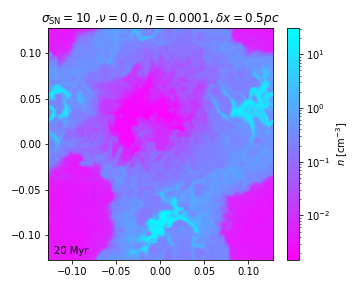
\includegraphics[trim=0.0cm 0.00cm 0.0cm 0.0cm,clip=true,width=0.33\textwidth]{csc_figs/rho05pcPm0e-4_02.png}
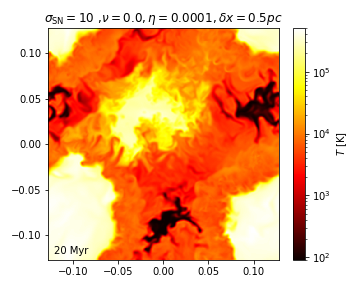
\includegraphics[trim=0.0cm 0.00cm 0.0cm 0.0cm,clip=true,width=0.33\textwidth]{csc_figs/tt05pcPm0e-4_02.png}
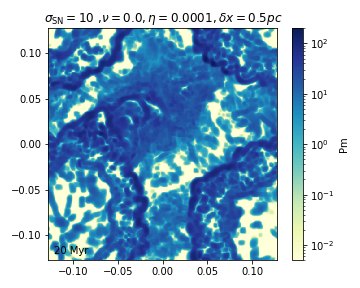
\includegraphics[trim=0.0cm 0.00cm 0.0cm 0.0cm,clip=true,width=0.33\textwidth]{csc_figs/Pm05pcPm0e-4_02.png}
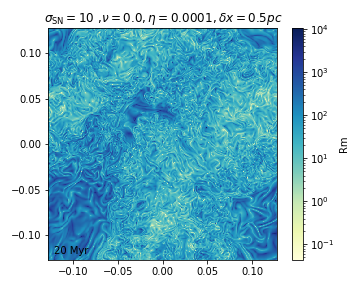
\includegraphics[trim=0.0cm 0.00cm 0.0cm 0.0cm,clip=true,width=0.33\textwidth]{csc_figs/Rm05pcPm0e-4_02.png}
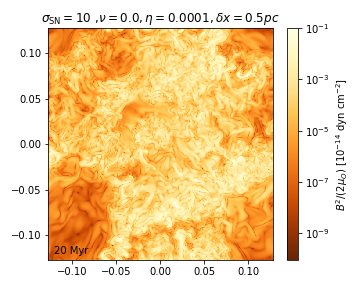
\includegraphics[trim=0.0cm 0.00cm 0.0cm 0.0cm,clip=true,width=0.33\textwidth]{csc_figs/pb05pcPm0e-4_02.png}
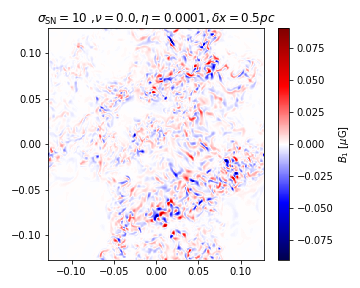
\includegraphics[trim=0.0cm 0.00cm 0.0cm 0.0cm,clip=true,width=0.33\textwidth]{csc_figs/bb105pcPm0e-4_02.png}
\caption{
Slices for resolution of 0.5\,pc with hyper diffusion coefficients as 
specified in Figure\,\ref{fig:brms}, and $\eta=10^{-4}$ sampled from the 
kinematic dynamo state.
\label{fig:05pcUB}
}
\end{figure*}
%--------------------------------------------------------------------------

%------------------------------------------------------------------------
\begin{figure*}
\centering
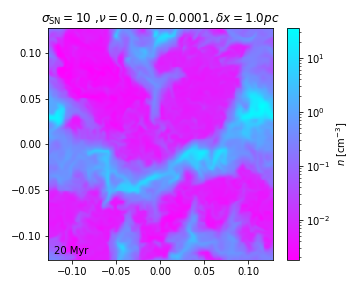
\includegraphics[trim=0.0cm 0.00cm 0.0cm 0.0cm,clip=true,width=0.33\textwidth]{csc_figs/rho1pcPm0e-4_00.png}
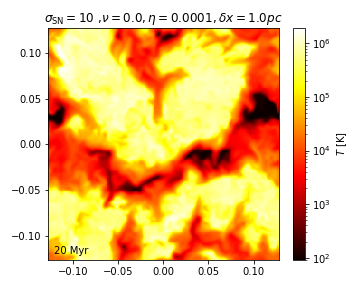
\includegraphics[trim=0.0cm 0.00cm 0.0cm 0.0cm,clip=true,width=0.33\textwidth]{csc_figs/tt1pcPm0e-4_00.png}
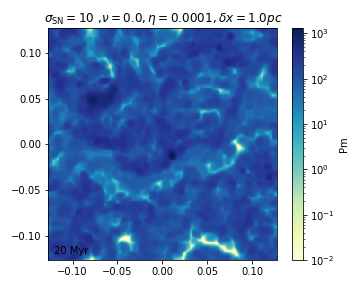
\includegraphics[trim=0.0cm 0.00cm 0.0cm 0.0cm,clip=true,width=0.33\textwidth]{csc_figs/Pm1pcPm0e-4_00.png}
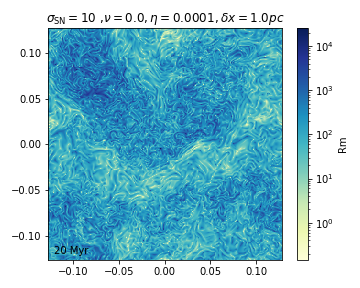
\includegraphics[trim=0.0cm 0.00cm 0.0cm 0.0cm,clip=true,width=0.33\textwidth]{csc_figs/Rm1pcPm0e-4_00.png}
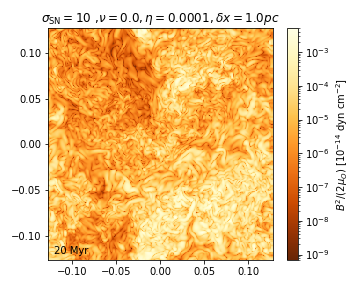
\includegraphics[trim=0.0cm 0.00cm 0.0cm 0.0cm,clip=true,width=0.33\textwidth]{csc_figs/pb1pcPm0e-4_00.png}
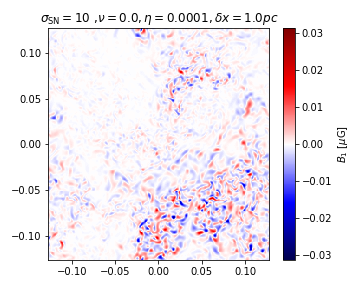
\includegraphics[trim=0.0cm 0.00cm 0.0cm 0.0cm,clip=true,width=0.33\textwidth]{csc_figs/bb11pcPm0e-4_00.png}
\caption{
Slices for resolution of 1\,pc with hyper diffusion coefficients as 
specified in Figure\,\ref{fig:brms}, and $\eta=10^{-4}$ sampled from the 
kinematic dynamo state.
\label{fig:1pcUB}
}
\end{figure*}
%--------------------------------------------------------------------------

%-------------------------------------------------------------------------
\begin{figure*}
\centering
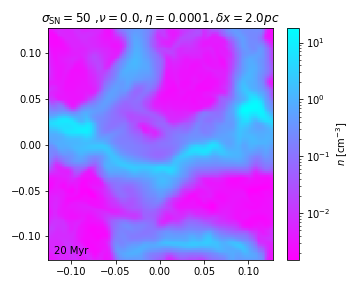
\includegraphics[trim=0.0cm 0.00cm 0.0cm 0.0cm,clip=true,width=0.33\textwidth]{csc_figs/rho2pcPm0e-4_00.png}
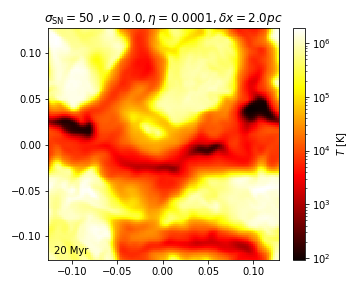
\includegraphics[trim=0.0cm 0.00cm 0.0cm 0.0cm,clip=true,width=0.33\textwidth]{csc_figs/tt2pcPm0e-4_00.png}
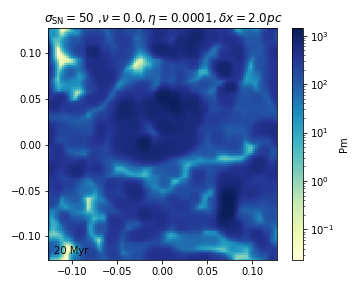
\includegraphics[trim=0.0cm 0.00cm 0.0cm 0.0cm,clip=true,width=0.33\textwidth]{csc_figs/Pm2pcPm0e-4_00.png}
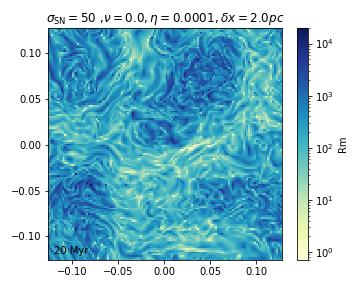
\includegraphics[trim=0.0cm 0.00cm 0.0cm 0.0cm,clip=true,width=0.33\textwidth]{csc_figs/Rm2pcPm0e-4_00.png}
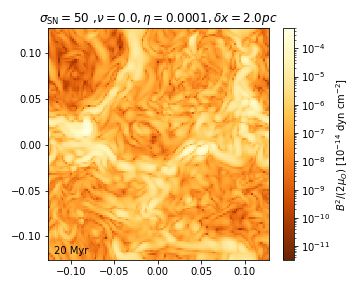
\includegraphics[trim=0.0cm 0.00cm 0.0cm 0.0cm,clip=true,width=0.33\textwidth]{csc_figs/pb2pcPm0e-4_00.png}
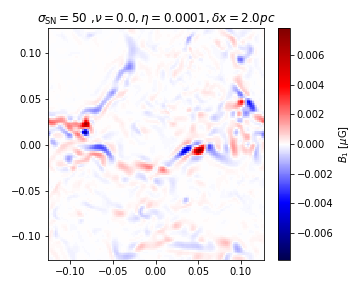
\includegraphics[trim=0.0cm 0.00cm 0.0cm 0.0cm,clip=true,width=0.33\textwidth]{csc_figs/bb12pcPm0e-4_00.png}
\caption{
Slices for resolution of 2\,pc with hyper diffusion coefficients as 
specified in Figure\,\ref{fig:brms}, and $\eta=10^{-4}$ sampled from the 
kinematic dynamo state.
\label{fig:2pcUB}
}
\end{figure*}
%--------------------------------------------------------------------------

%-------------------------------------------------------------------------
\begin{figure*}
\centering
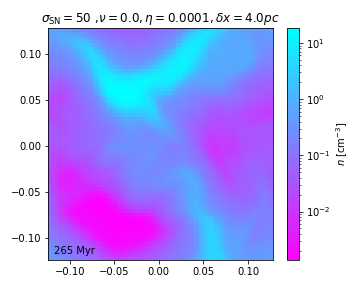
\includegraphics[trim=0.0cm 0.00cm 0.0cm 0.0cm,clip=true,width=0.33\textwidth]{csc_figs/rho4pcPm0e-4_032.png}
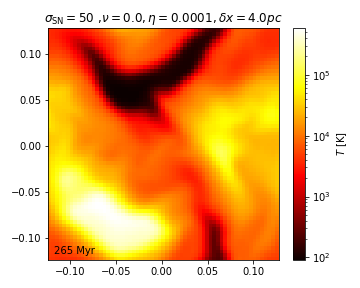
\includegraphics[trim=0.0cm 0.00cm 0.0cm 0.0cm,clip=true,width=0.33\textwidth]{csc_figs/tt4pcPm0e-4_032.png}
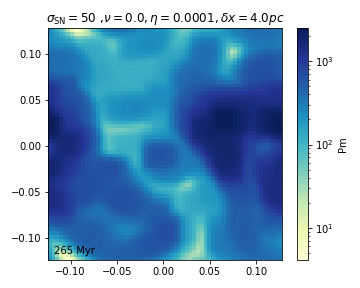
\includegraphics[trim=0.0cm 0.00cm 0.0cm 0.0cm,clip=true,width=0.33\textwidth]{csc_figs/Pm4pcPm0e-4_032.png}
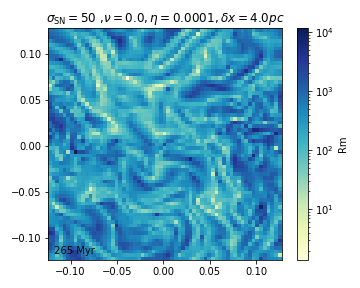
\includegraphics[trim=0.0cm 0.00cm 0.0cm 0.0cm,clip=true,width=0.33\textwidth]{csc_figs/Rm4pcPm0e-4_032.png}
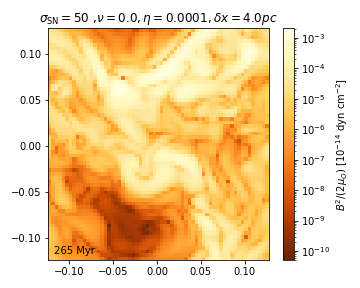
\includegraphics[trim=0.0cm 0.00cm 0.0cm 0.0cm,clip=true,width=0.33\textwidth]{csc_figs/pb4pcPm0e-4_032.png}
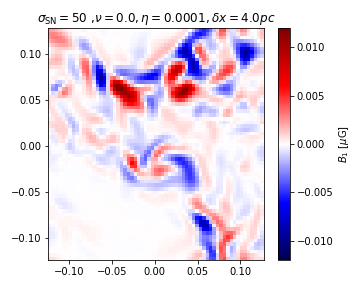
\includegraphics[trim=0.0cm 0.00cm 0.0cm 0.0cm,clip=true,width=0.33\textwidth]{csc_figs/bb14pcPm0e-4_032.png}
\caption{
Slices for resolution of 4\,pc with hyper diffusion coefficients as 
specified in Figure\,\ref{fig:brms}, and $\eta=10^{-4}$ sampled from the 
kinematic dynamo state.
\label{fig:4pcUB}
}
\end{figure*}

%--------------------------------------------------------------------------
\section{Helmhlotz decomposition test sample}
%-------------------------------------------------------------------------
\begin{figure*}
\centering
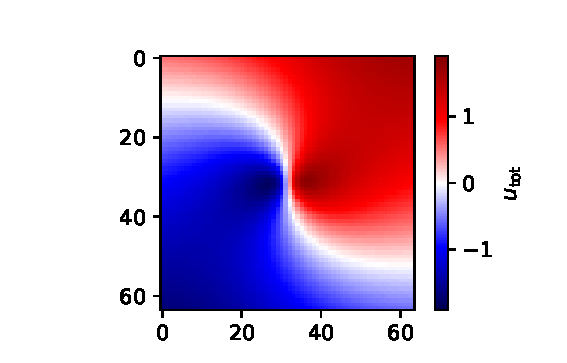
\includegraphics[trim=0.4cm 0.0cm 0.0cm  0.0cm,clip=true,height=0.22\textwidth]{csc_figs/helm_test1.eps}
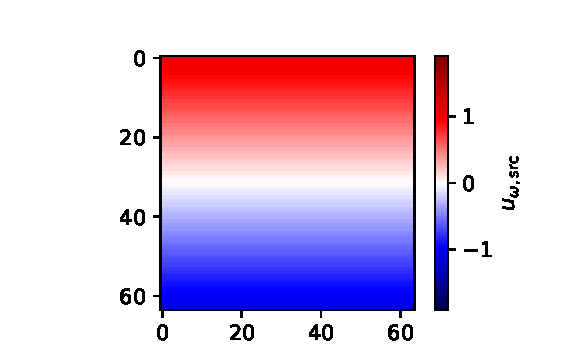
\includegraphics[trim=1.0cm 0.0cm 0.0cm  0.0cm,clip=true,height=0.22\textwidth]{csc_figs/helm_test2.eps}
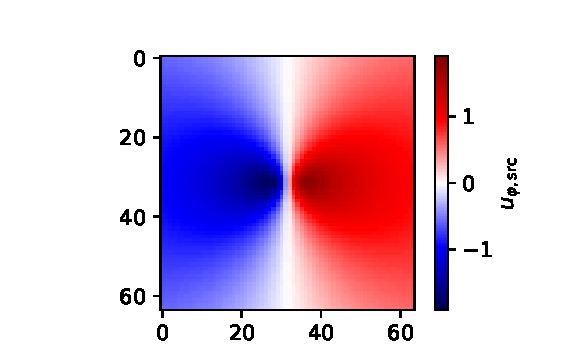
\includegraphics[trim=1.0cm 0.0cm 0.0cm  0.0cm,clip=true,height=0.22\textwidth]{csc_figs/helm_test4.eps}
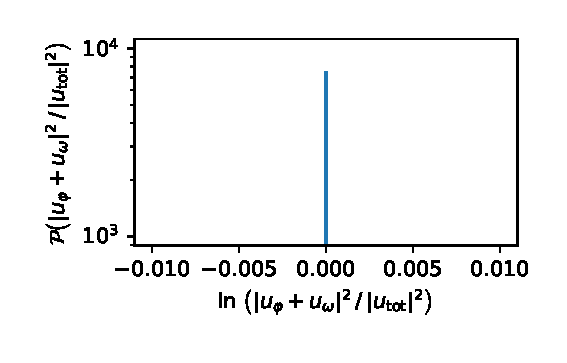
\includegraphics[trim=0.4cm 0.3cm 0.2cm -0.2cm,clip=true,height=0.22\textwidth]{csc_figs/helm_hist.eps}
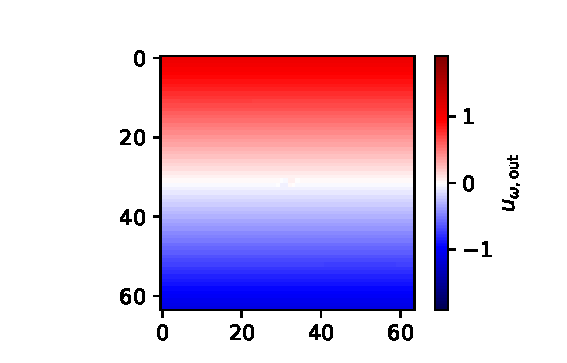
\includegraphics[trim=1.0cm 0.0cm 0.0cm  0.0cm,clip=true,height=0.22\textwidth]{csc_figs/helm_test3.eps}
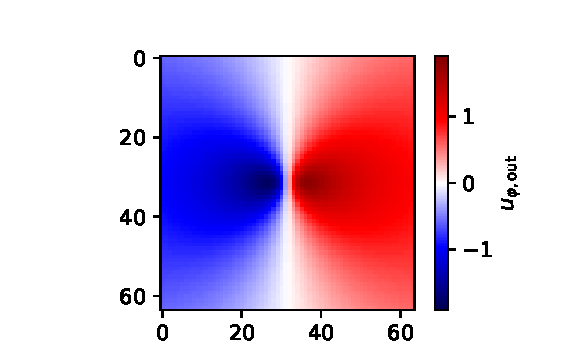
\includegraphics[trim=1.0cm 0.0cm 0.0cm  0.0cm,clip=true,height=0.22\textwidth]{csc_figs/helm_test5.eps}
\caption{
Test flow, panel {\bf{(a)}}, comprising sum of rotational flow, panel
{\bf{(b)}}, and potential flow, panel {\bf{(c)}}, applying the Helmholtz
decomposition result in panels {\bf{(e)}} and {\bf{(f)}}.
The PDF of the ratio of decomposed internal energy summed to total internal
energy returns a $\delta$-function, indicative of orthogonal solutions.
\label{fig:helm_test}
}
\end{figure*}
%--------------------------------------------------------------------------

%-------------------------------------------------------------------------
\begin{figure*}
\centering
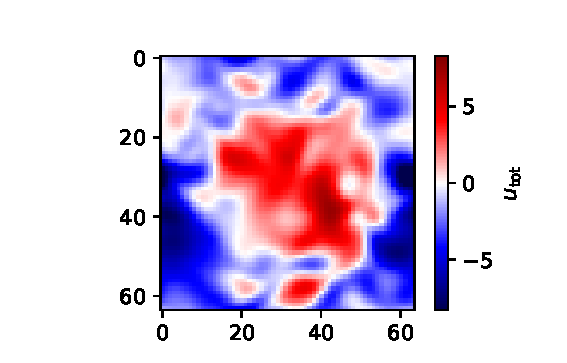
\includegraphics[trim=0.4cm 0.0cm 0.0cm  0.0cm,clip=true,height=0.22\textwidth]{csc_figs/helm_sim1.eps}
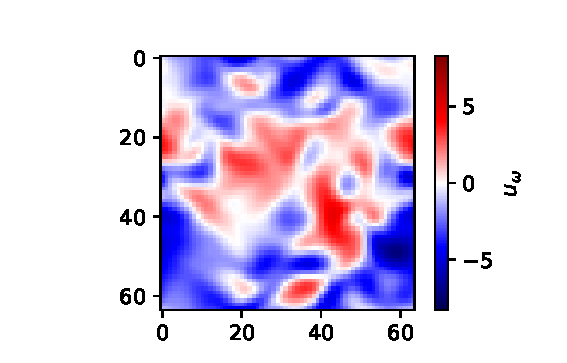
\includegraphics[trim=1.0cm 0.0cm 0.0cm  0.0cm,clip=true,height=0.22\textwidth]{csc_figs/helm_sim2.eps}
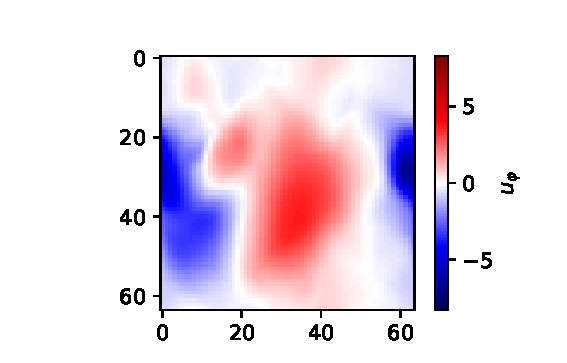
\includegraphics[trim=1.0cm 0.0cm 0.0cm  0.0cm,clip=true,height=0.22\textwidth]{csc_figs/helm_sim3.eps}
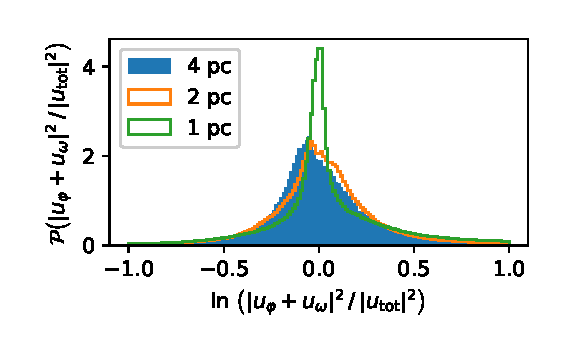
\includegraphics[trim=0.4cm 0.3cm 0.2cm -0.2cm,clip=true,height=0.22\textwidth]{csc_figs/helm_hsim.eps}
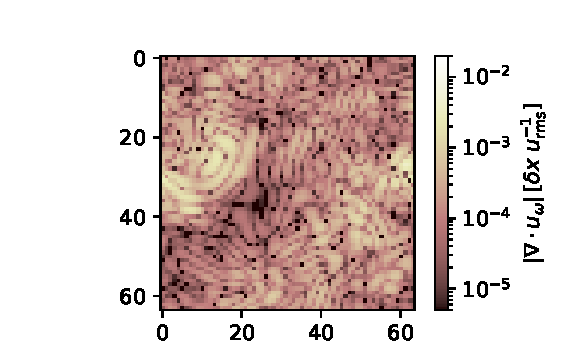
\includegraphics[trim=1.0cm 0.0cm 0.0cm  0.0cm,clip=true,height=0.22\textwidth]{csc_figs/helm_divu.eps}
\includegraphics[trim=1.0cm 0.0cm 0.0cm  0.0cm,clip=true,height=0.22\textwidth]{csc_figs/helm_curl.eps}
%\includegraphics[trim=1.0cm 0.0cm 0.0cm 0.0cm,clip=true,width=0.3\textwidth]{csc_figs/helm_temp.eps}
\caption{
Simulation flow, panel {\bf{(c)}}, applying the Helmholtz decomposition result
in panels {\bf{(b)}} and {\bf{(c)}}.
The non-zero divergence of the rotational portion, {\bf{(d)}}, and curl of the
potential portion, {\bf{(e)}}, indicate the extent to which the discrete 
decomposition is not orthogonal due to extreme gradients.
Temperature, {\bf{(f)}}, is included to show how these extrema align with ISM phase.
\label{fig:helm_sim}
}
\end{figure*}
%--------------------------------------------------------------------------

%--------------------------------------------------------------------------
\begin{table*}[h]
\begin{tabular}{ccl}
\hline\hline\\
{Notation Symbol} & {Denoting} & {Units/Definition}\\\hline\\
 $\dfrac{D}{Dt}$ & material derivative & $\dfrac{\partial }{\partial t}+\vect{u}\cdot \vect\nabla$ \\
 $\vect\nabla$ & gradient vector & e.g., $\left(\dfrac{\partial }{\partial x},\dfrac{\partial }{\partial y},\dfrac{\partial }{\partial z}\right)$ \\
 $\rho$ & gas density & [g cm$^{-3}$]  \\
 $\vect u$ & gas velocity & [km s$^{-1}$] \\
 $t$ & time & [Myr] \\
 $s$ & specific entropy & [erg g$^{-1}$ K$^{-1}$] \\
 $T$ & gas temperature & [K] \\
 $\vect A$ & magnetic vector potential & [$\upmu$G cm] \\
 $\vect B$ & magnetic field & [$\upmu$G] \\
 $\vect j$ & current density & [Bi cm$^{-2}$] \\
 $\mathbfss W$ & traceless rate of strain tensor &
   ${\mathsf W}_{ij} = \dfrac{1}{2}\left(\dfrac{\partial u_i}{\partial x_j}
                  + \dfrac{\partial u_j}{\partial x_i}
                  -\dfrac{2}{3} \delta_{ij}\vect\nabla\cdot \vect u\right)$ \\
 $|\mathbfss W|^2$ & contracted rate of strain tensor &
   $|\mathbfss W|^2={\mathsf W}_{ij}{\mathsf W}_{ij}$\\
 $\mathbfss W^{(3)}$ & 6th order rate of strain tensor &
   ${\mathsf W}_{ij}^{(3)} = \dfrac{1}{2}\left(\dfrac{\partial^5 u_j}{\partial x_i^5}
                  + \dfrac{\partial^4}{\partial x_i^4}\left(\dfrac{\partial u_i}{\partial x_j}\right)
                  -\dfrac{1}{3}\dfrac{\partial^4}{\partial x_i^4}\left(\vect\nabla\cdot \vect u\right)\right)$ \\
 $\zeta_{D},\zeta_{\nu},\zeta_{\chi}$ & shock diffusion coefficient& $\propto \left(-\vect\nabla\cdot\vect u\right)_+$\\
 $\nu,\eta$ & viscosity, resistivity coefficient& [kpc km s$^{-1}$]\\
 $\nu_3,\chi_3,\eta_3$ & hyperdiffusion coefficient& [kpc$^{5}$ km s$^{-1}$]\\
 $\Gamma$ & UV-heating& [erg g$^{-1}$ s$^{-1}$]\\
 $\Lambda$ & radiative cooling& [erg cm$^{3}$ g$^{-2}$ s$^{-1}$]\\
 $\ESK+\EST$ & SN explosion energy& [10$^{51}$erg]\\
 $\dot\sigma$ & SN explosion rate & [kpc$^{-3}$ Myr$^{-1}$]\\
 $c_{\rm s}$ & sound speed & [km s$^{-1}$]\\
 $c_{\rm p}$ & specific heat at constant pressure & [erg g$^{-1}$ K$^{-1}$]\\
 $e_B$ & magnetic energy density & [erg cm$^{-3}$]\\
 $\overline{e_K}$ & time-averaged kinetic energy density & [erg cm$^{-3}$]\\
\hline
\end{tabular}
\end{table*}


\section{Conclusions}\label{sec:conc}

\acknowledgments
 {We thank O. Gressel and D. Elstner for discussions inspiring this work,
 and the anonymous referee for comments producing substantial improvement of
 the presentation.}
 F.A.G. and M.J.K. acknowledge support from the Academy of Finland
 ReSoLVE Centre of Excellence (grant 307411) and the ERC
 under the EU's Horizon 2020 research and innovation
 programme (Project UniSDyn, grant 818665) and generous computational
 resources from CSC -- IT Center for Science, Finland, under Grand
 Challenge GDYNS Project 2001062. 
 M-M.M.L. was partly supported by US NSF grant AST18-15461.

\software{Pencil Code \citep{brandenburg2002,Pencil-JOSS}}

\bibliographystyle{aasjournal}
\bibliography{refs}{}
\newpage
\section*{simulation notes}

Summary of open notes from previous meetings
\begin{itemize} 
\item compare thermal runaway with Li \& Ostriker 
\item include spectra during growth with time evolution (hot vs cold)
\item use auto-correlation functions to determine typical velocity per phase
\item see Chira et al / Mac Low
\item compare helicity for varying local gamma
\item Scale of dynamo forcing may not be the scale of the SN bubbles? Peak of magnetic energy spectrum may be the relevant scale
\item Compare peak $k$ of $P_B(k)$, is $\eta\propto\ell^2$?
\item apply Helmholtz decomposition to the total flow. Compare vorticity in hot
phase prior to and during the dynamo epoch. Is there a jump in vorticity in the
hot gas? How is this evolving in the warm gas related to the dynamo state? 
Vorticity has been demonstrated to strongly affect SSD in other systems.
\item use auto-correlation functions to determine typical velocity per phase.
Does James' method account for the discontinuous volume of the hot gas to
recover the relevant correlation length by phase? Check references/Anvar?
Divide out volume correlation function from correlation function of phase?
\item $k^{3/2}$ not obeyed at low $k$ - does this correspond to bubble size?
Auto-correlation analysis to compare $\ell$ with bubble size $L_{\rm SN}$
and $k$-space.
Power laws fit well for magnetic but not kinetic.
Is this due to two dynamos?
Separate hot amd warm gas to investigate spectra and auto-correlation.
\item correlation functions - divide out corr function by volume to obtain phase?
\item include error bars for variance of orthogonality by point
\item what is the error in div/curl
\end{itemize}

\end{document}

